\documentclass[a4paper,12pt, headsepline]{scrartcl}

\usepackage[utf8]{inputenc}
\usepackage[T1]{fontenc}
\pagestyle{plain}
\usepackage{lmodern}
\usepackage[english]{babel}
\usepackage[official]{eurosym}
\usepackage{ntheorem}
\newtheorem{hyp}{Hypothesis}
\usepackage{pdfpages}
\usepackage{adjustbox}
\usepackage{footnote}
\usepackage{filecontents}
\usepackage{titling}
\usepackage{csquotes}
\usepackage[objectset = centering]{floatrow}
\usepackage{moreverb}
\usepackage{varioref}
\usepackage{setspace}
\usepackage{graphicx}
\usepackage{tabularx}
\usepackage{dcolumn}
\usepackage{float}
\usepackage{color}
\usepackage{amsmath} 
\usepackage{float}
\usepackage[
colorlinks = true,
linkcolor = black,
citecolor = blue 
]{hyperref}

\setlength{\parindent}{0ex} 
\setlength{\parskip}{1ex}


\usepackage[automark]{scrlayer-scrpage}
\setkomafont{pagehead}{\scshape}
\pagestyle{scrheadings}
\ihead{\headmark}
\chead{}
\ohead{}

\cfoot{\pagemark}


\usepackage{csquotes}
\usepackage[
backend=biber,
natbib=true,
language = english,
doi = false, url = false, isbn = false, eprint = false,
style = apa]
{biblatex}
\DeclareLanguageMapping{english}{english-apa}
\addbibresource{literature.bib}

% Schrift
\setkomafont{sectioning}{\rmfamily\bfseries\boldmath}

\setcapindent{0em} % kein Einrücken der Caption von Figures und Tabellen
\setcapwidth{0.9\textwidth} % Breite der Caption nur 90% der Textbreite, damit sie sich vom restlichen Text abhebt
\setlength{\abovecaptionskip}{0.2cm} % Abstand der zwischen Bild- und Bildunterschrift
\renewcommand{\baselinestretch}{1.5}
\numberwithin{equation}{section}
\title{Predicting Award Prices of First Price Sealed Bid Procurement Auctions}
\date{07/14/2022}
\author{Fabian Blasch\\[0.4cm]{Supervisor: Dr. Katharina Fenz}}
\begin{document}
\begin{titlingpage}
\maketitle
\end{titlingpage}
\newpage
\tableofcontents
\thispagestyle{empty}
\clearpage
\pagenumbering{arabic} 

\section{Introduction}\label{sec:int}

\section{Data}\label{sec:data}

All the information about the procurement contracts, is obtainable through the bid tab archive on the official website of the Colorado Department of Transportation. The information is provided in PDF documents. In each of those documents the following information of the respective auction is provided.

\begin{itemize}
	\item A table listing all submitted bids, including a unique identifier for each of the participating bidders
	\item A contract description
	\item An engineer's estimate
	\item The contract ID
	\item The letting date
	\item Either the amount of time in business days given to complete all the contractual obligations, or a completion due date
	\item The county in which the contract is to be completed in 
\end{itemize}

For illustrative purposes, Figure \ref{fig:bidtab} displays an example of a bid tab, in particular the second page, which contains the vendor ranking as well as the contract description and the remaining information listed above.

\begin{figure}[H]
	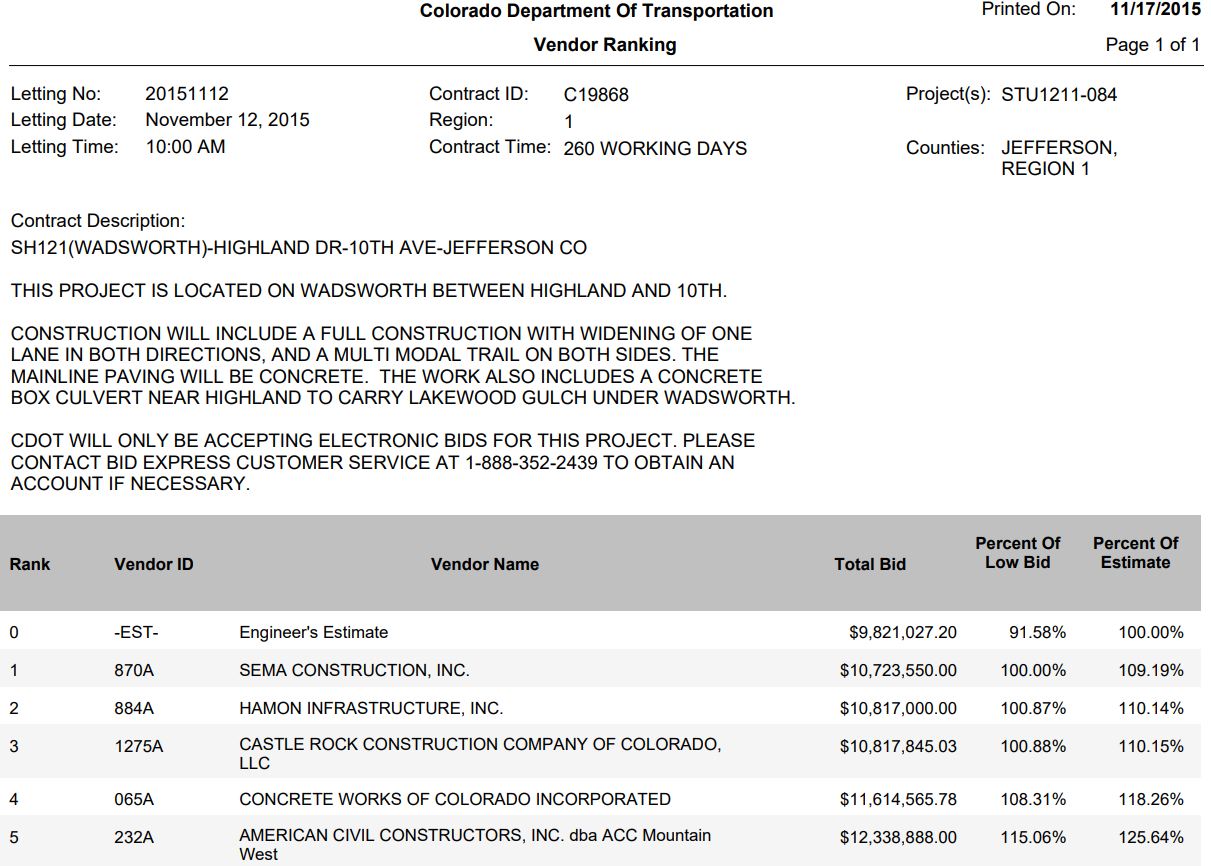
\includegraphics[width = 14	cm]{figures/Bid_Tab_exmpl.PNG}
	\caption{Bid Tab Example}\label{fig:bidtab}
\end{figure}

\subsection{Scraping}\label{subsec:scrap}
In order to obtain all the archived bid tabs, the html code of the website was first examined using a google chrome extension called SelectorGadget. This tool allows one to identify html nodes, that website contents are associated with. In the case of the bid tab archive, the html node carrying the links to the individual bid tabs is \enquote{<td a>}. Once this html node is discovered and the consistency across different years in the archive is ensured, the download is easily achieved by looping over the links and downloading the  respective PDF. The hyperlink extraction was performed utilizing \textit{rvest}, by \citet{rvest}. For the remaining steps in the data extraction process, a distinction will be made for text based information and tabular data.

\subsubsection{Text Based Information}\label{subsubsec:descr}
 The structure of the text based information allows us to filter the individual parts via regular expressions. Especially, for the letting data, the contract ID, and the county this required no further data cleaning steps. Unfortunately, this is not the case for the contract time and the contract description.\\ 
 The contract time was not as straightforward to obtain, since the way it is reported is inconsistent across documents. Most of the time it is reported as working days until all contractual obligations have to be fullfilled. Seldom, however, the bid tab contains a completion date instead. Accordingly, to achieve consistency across documents all completion dates were converted to contract time. This was achieved by first adding 60 days to the letting date, as this is the number of days that the Cdot reports as the expected time between the letting date and the start of the work on site. Then, the difference in days between the completion date and the starting date were computed. As, said difference is only supposed to contain working days the following holidays as well as all weekends were substracted from the difference betwen starting date and completion date.
 
 \begin{itemize}
 	\item New Year's Day
 	\item Dr. Martin Luther King, Jr. Day
 	\item President's Day
 	\item Memorial Day
 	\item Juneteenth
 	\item Independence Day
 	\item Labor Day
 	\item Frances Xavier Cabrini Day
 	\item Veterans Day
 	\item Thanksgiving
 	\item Christmas
 \end{itemize}
 
 The computation was executed utilizing the R package \textit{bizdays}, \citet{bizdays}. The package enables the user to generate custom calenders. The difference in starting and completion date was therefore easily calculated by setting up a custom calender with the holidays listed above as well as all saturdays and sundays. Then using this calender, the difference between two dates will only take working days into account.
 The only remaining text based information is the contract description. So far none of the text based information required extensive preprocessing to obtain variables that can be represented in a tabular format. In the case of the contract description this is not the case. In order to convert the contract description into a format that may be represented in a table, the descriptions were first tokenized. Tokenization refers to splitting the input text into single unique words, i.e., splitting the sentences on spaces and removing all forms of punctuation. The result is then a vector of tokens. Said tokens were then scanned for spelling mistakes utilizing the R package \textit{hunspell} \citep{hunspell}. Once the misspelled words were corrected, stopwords were removed from the list of tokens. Stopwords are words that have no inherent signal associated with their use, examples for such words in the english language would be \enquote{a}, \enquote{is} and \enquote{the}. In natural language processing there is not necessarily one list of stopwords, depending on the context different libraries of stopwords may be used to remove as much noise as possible from textual data while leaving the signal associated with a series of words in tact. In the case of this thesis, a combination of five different libraries of stopwords was used. All of those libraries, \enquote{snowball} , \enquote{stopwords-iso}, 
 \enquote{smart}, \enquote{marimo} and \enquote{nltk} are available through the R package \textit{stopwords}, by \citet{stopwords}. After filtering out the stopwords, the remaining words were then stemmed.
 
 
 
\begin{figure}[H]
	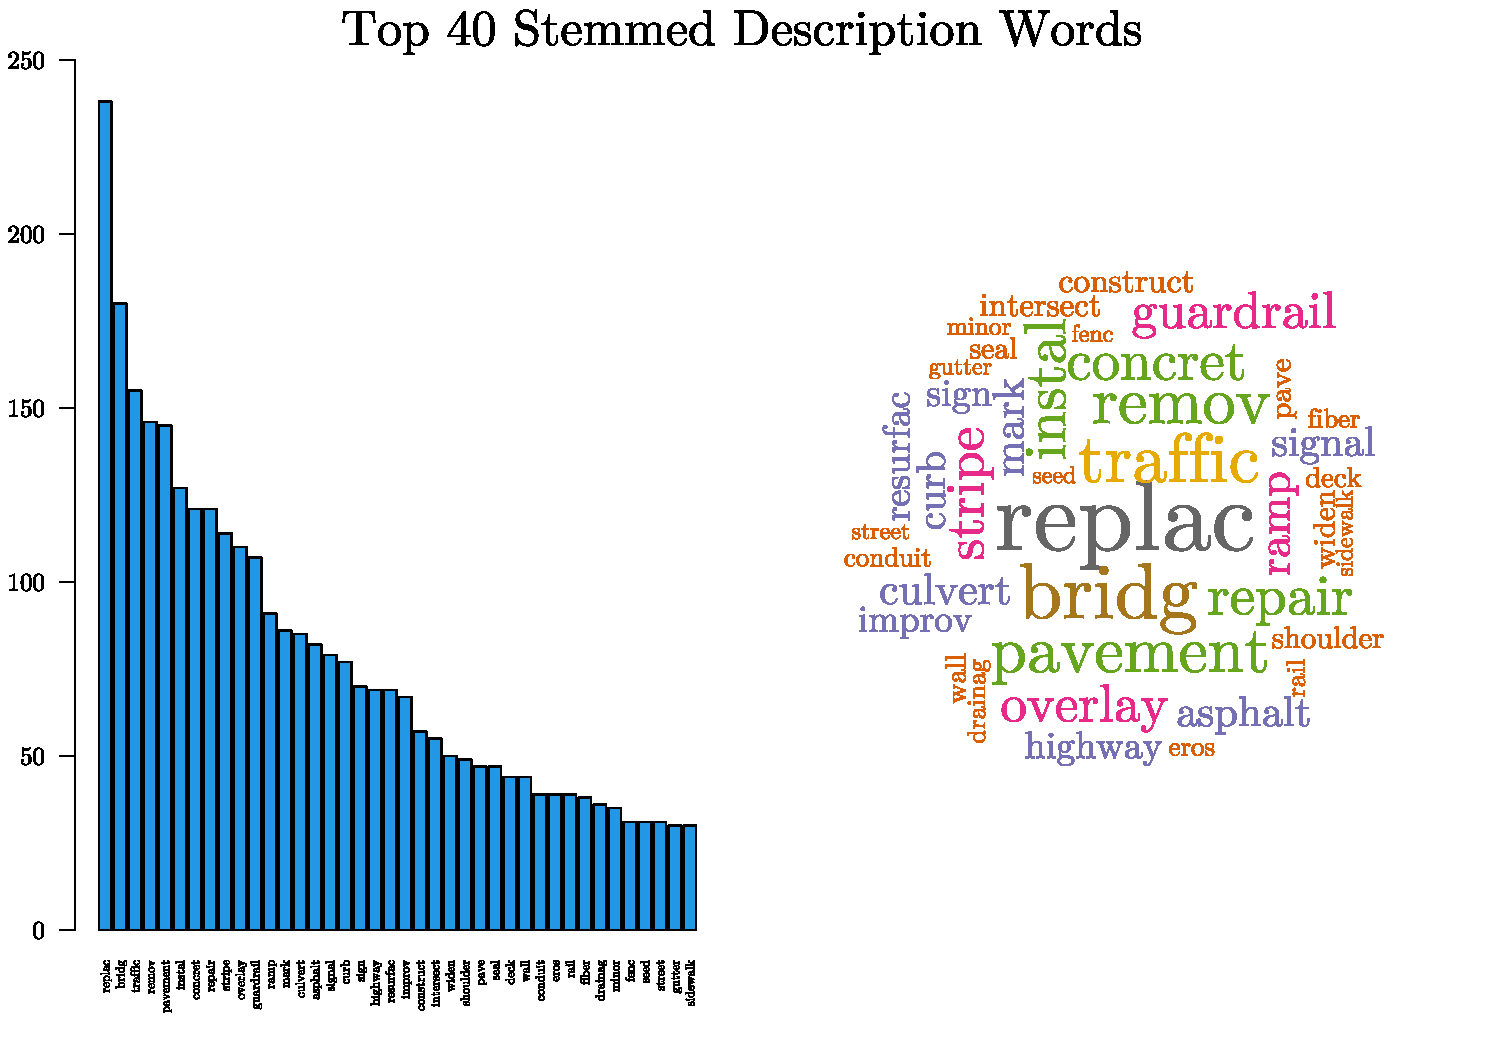
\includegraphics[width = 14	cm]{figures/description_words.pdf}
	\caption{Top 40 Stemmed Description Words}\label{fig:desc}
\end{figure}

\subsection{Descriptive Statistics}\label{subsec:desc}
\section{Economic Operationalization}\label{sec:op}
\subsection{Auctioneer}\label{subsec:auc}
\subsection{Firms}\label{subsec:firms}

\section{Methods}\label{sec:meth}
\subsection{Elastic Nets}\label{subsec:net}
\subsection{Ensemble Methods}\label{subsec:ens}
\subsubsection{Random Forests}\label{subsubsec:rf}
\subsubsection{eXtreme Gradient Boosting}\label{subsubsec:xgb}
\subsection{Nested Cross Validation}\label{subsec:nest}
\subsubsection{Logistic PCA}\label{subsubsec:logp}
\subsubsection{Recursive Feature Elimination}\label{subsubsec:rfe}
\section{Results}\label{sec:res}
\subsection{Prediction}\label{subsec:pred}
\subsection{Unsupervised Colusion Detection}\label{subsec:col}
\section{Conclusion}\label{sec:con}
 
\newpage
\printbibliography

\end{document}